Alice wirft einen Stein von einem Aussichtsturm.
\smallskip

\begin{minipage}{0.2\textwidth}
    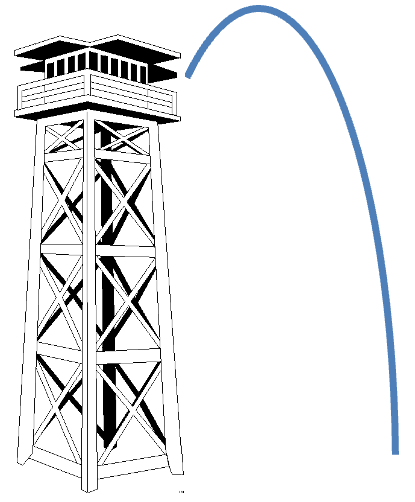
\includegraphics[width=\textwidth]{Einführung/im/Aussichtsturm.png}
\end{minipage}
\begin{minipage}{0.8\textwidth}
    Die Flugphase des Steins kann durch die folgende Funktion beschrieben werden:
    \[h(t)=-5t^2+5t+30\]
    Dabei ist $h(t)$ die Höhe des Steins über dem Boden (in Meter) und $t$ bezeichnet die Zeit, die seit dem Abwurf verstrichen ist (in Sekunden).
\end{minipage}
\begin{enumerate}
    \item Vervollständigen Sie die Wertetabelle:
          \begin{tabular}{|c|c|c|c|c|c|c|c|}
              t & $0$ & $0.5$ & $1$ &
          \end{tabular}
\end{enumerate}